\section{Intelligenza artificiale }
Con intelligenza artificiale intendiamo le metodologie e le tecniche che consentono la progettazione di sistemi hardware e sistemi di programmi software capaci di fornire all'elaboratore elettronico prestazioni che, a un osservatore comune, sembrerebbero essere di pertinenza esclusiva dell’intelligenza umana
(Marco Somalvico).La nascita effettiva di questa disciplina è da ricercarsi nei lavori di John McCarthy, Marvin Minsky, Claude Shannon e Nathaniel Rochester \cite{McCarthy_Minsky_Rochester_Shannon_2006} dei primi anni 50 ,mentre il primo software che conteneva caratteristiche tali da poterne fare  parte fu il Logic Theorist, o LP che permetteva di dimostrare semplici teoremi matematici partendo dai prinicipi del calcolo , di di Allen Newell e Herbert Simon \cite{10.1145/1455567.1455605},negli anni successivi lo sviluppo cominicio ad entrare nell'industria , fino ai tempi moderni nei quali i termini AI e inteligenza artificiale sono diventati di uso comune e di forte potere mediatico .


\subsection{ Il Deep Lerning e le reti neurali artificiali  }
Le reti neurali artificiali cercano di emulare il funzionamento delle interazioni tra neuroni all’interno di un cervello umano. Semplificandone il processo, sono stati definiti dei modelli dedicati a diversi tipi di problemi, tra cui il riconoscimento di pattern, il clustering e  la predizione. 
Con  Deep Learning,(Aprendimento profondo ) si intende quella branchia dell'inteligenza artificiale e dell'apprendimento automatico nella quale si utilizzano reti neurali artificiali per svolgere calcoli;
tutto cio è possibile grazie all' utilizzo di modelli gerarchici che rappresentano distribuzioni di probabilità su dati quali immagini, conversazioni audio, e testo.
L’obiettivo ultimo di un progetto di Deep Learning è sviluppare un modello che rappresenti una certa realtà: un’immagine, un testo, etc.
Quindi si parte dall'analisi dei dati , di cui disponiamo, si stabiliscono  delle funzioni matematiche e attraverso iterazioni successive e l’ausilio dell algoritmica , ricaviamo i parametri che definiscono la funzione e di conseguenza il modello.
\subsubsection{Reti neurali}
Una rete di neuroni  può essere intesa come un grafo pesato, in cui i singoli neuroni(nodi del grafo) sono collegati tra di loro con archi orientati e pesati . I nodi vengono organizzati in più strati quelli di  ingresso, strati  nel mezzo chiamati  “hidden” cioè nascosti e quelli di uscita, che formano un sistema in grado di fornire output partendo da  dati in input.\\
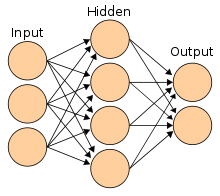
\includegraphics[]{reteneurale}\\
Ogni neurone calcola la somma pesata dei suoi dati in ingresso, a cui viene poi applicata la funzione di attivazione  tipica dello strato. Passando da neurone a neurone e da strato a strato a seconda del modello della rete neurale ci sarà quindi un valore di uscita con  dimensioni conformi della grandezza dello strato di output.


Lo scopo del sistema è quello di porre la questione come un problema di minimo. Se il problema è posto correttamente e la rete neurale è sufficientemente grande (anche se questo vale solo per strati densi, di cui parleremo dopo), si verificherà una discesa del gradiente (13) cercando di avvicinarsi al minimo, con un errore calcolato tramite la funzione di costo. Nel corso dell’allenamento (quindi della ricerca del minimo) ogni errore viene valutato tramite l’algoritmo di back-propagation e i pesi del grafo vengono aggiornati in base a questo. Un sistema di questo tipo che riesce a identificare uno o più minimi si dice che “converge” verso la soluzione ideale.

\subsection{Le Gan}

Una delle più recenti  e interessanti  applicazioni delle reti neurali sono le “reti generative avversarie” (Generative Adversarial Networks, abbreviato come GAN), che saranno il fulcro di questa trattazione . Questo tipo di rete neurale è specializzata nella generazione di dati e si avvale di due reti appunto “avversarie” nel loro scopo: la prima genererà un set di informazioni, l’altra dovrà classificare queste informazioni tra un set di “reali” e un set di “non reali”, cioè generate. Nel caso in cui la rete discriminatrice riesca effettivamente a riconoscere il tipo di dato avrà avuto successo a discapito della generatrice. In questo modo le reti si addestrano e migliorano  man mano che l’allenamento procede, registrando i pattern utilizzati allo scopo di generare output sempre migliori per la generatrice o riuscire a riconoscere sempre meglio quelli generati per quanto riguarda l’altra. Lo scopo è di riuscire a potenziare la rete generatrice fino a che la rete discriminatrice non riesca più a trovare differenze tra i dati generati e quelli posti in input. A questo punto, premesso il corretto funzionamento del sistema, la rete sarà in grado di generare dati estremamente convincenti.
Molto spesso i sistemi GAN sono pensati per generare immagini. Ce ne sono state moltissime declinazioni nel tempo, ognuna con la propria utilità. Partendo dalle più basilari capaci di generare cifre scritte a mano da pochi pixel di dimensione, si arriva alle più recenti adibite alla generazione di paesaggi in alta risoluzione o addirittura volti, considerati oggetti molto complessi per una grande varietà di motivi.
Lo scopo di questo progetto sarà progettare una GAN che possa lavorare con frasi reali e descrittive. In particolare, la GAN verrà allenata con dataset di uccelli e fiori 




\subsubsection{Generatore }
Il Generatore si occupa della generazione dei dati partendo dalla sorgente o dai dati in ingresso  in generale il processo di generazione è molto simile a quello che troviamo nelle Cnn (Reti neurali convoluzionali) per le GAN si ha  un ventaglio di architetture tipicamente usate(cosi come  per le Cnn). Una di queste è la DCGAN, una delle più popolari per la rete generativa.
Attraverso convoluzioni multiple trasposte eseguiamo l’upsampling da un generico ingresso o rumore (lo indicheremo con Z)  per generare un set di dati (che indicheremo con  X).\\
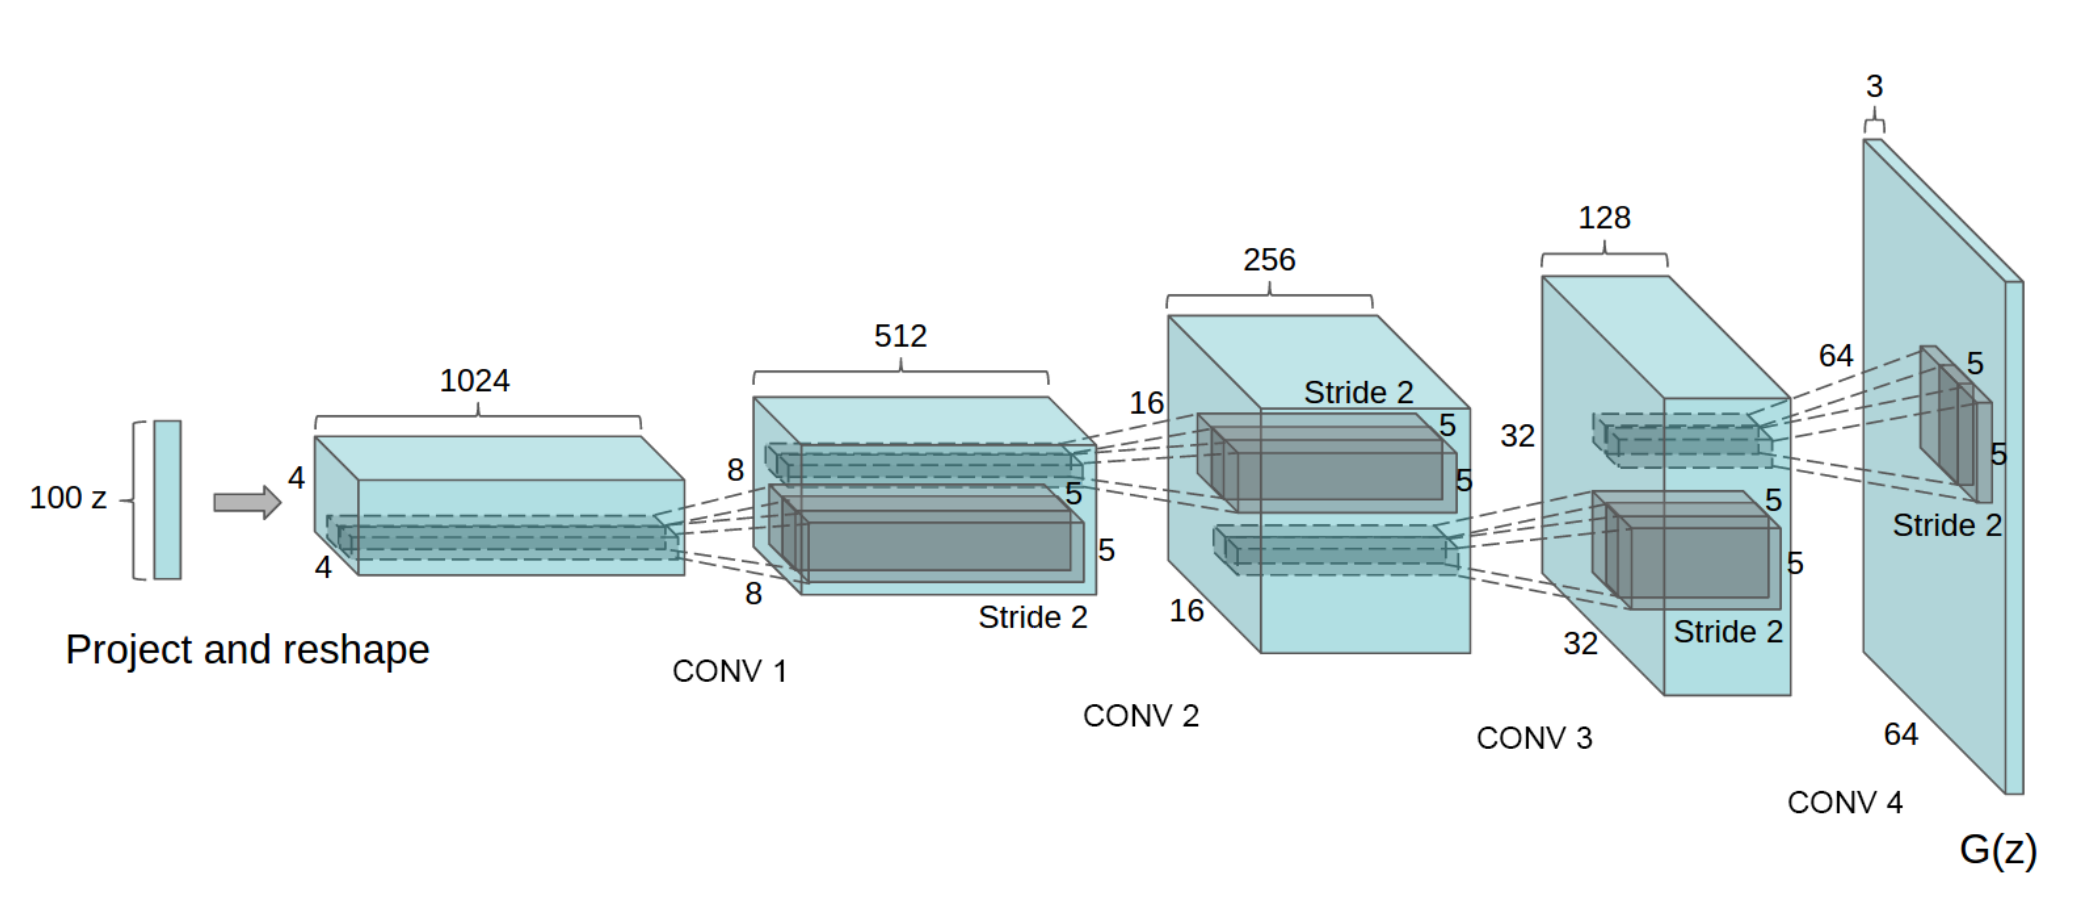
\includegraphics[scale=0.20]{gernerator}


\subsubsection{Discriminatore}
Un  generatore da solo creerebbe solamente dei dati sui quali non potremmo dire nulla ;
a questo punto dobbiamo introdurre il discriminatore ovvero quella rete neurale  che si occupa di distinguere i dati plausibili con quelli che non lo sono ;diamo quindi come input al discriminatore l'output del generatore e lo confrontiamo con i dati presenti nel dataset .
Il Discriminator esamina quindi i dati  reali (del dataset di training) e genera immagini separatamente.
Produce una probabilità D(x) compresa tra 0 e 1 che il dato in input sia reale o fittizio, a questo punto il discriminatore sancisce l' autenticita o meno del dato 

\subsection{Retropropagazione dell'errore e training}
Entriamo ora nel vivo dell'apprendimento ogni esecuzione delle due reti neurali genera quindi 


 \subsection{AttnGan}
 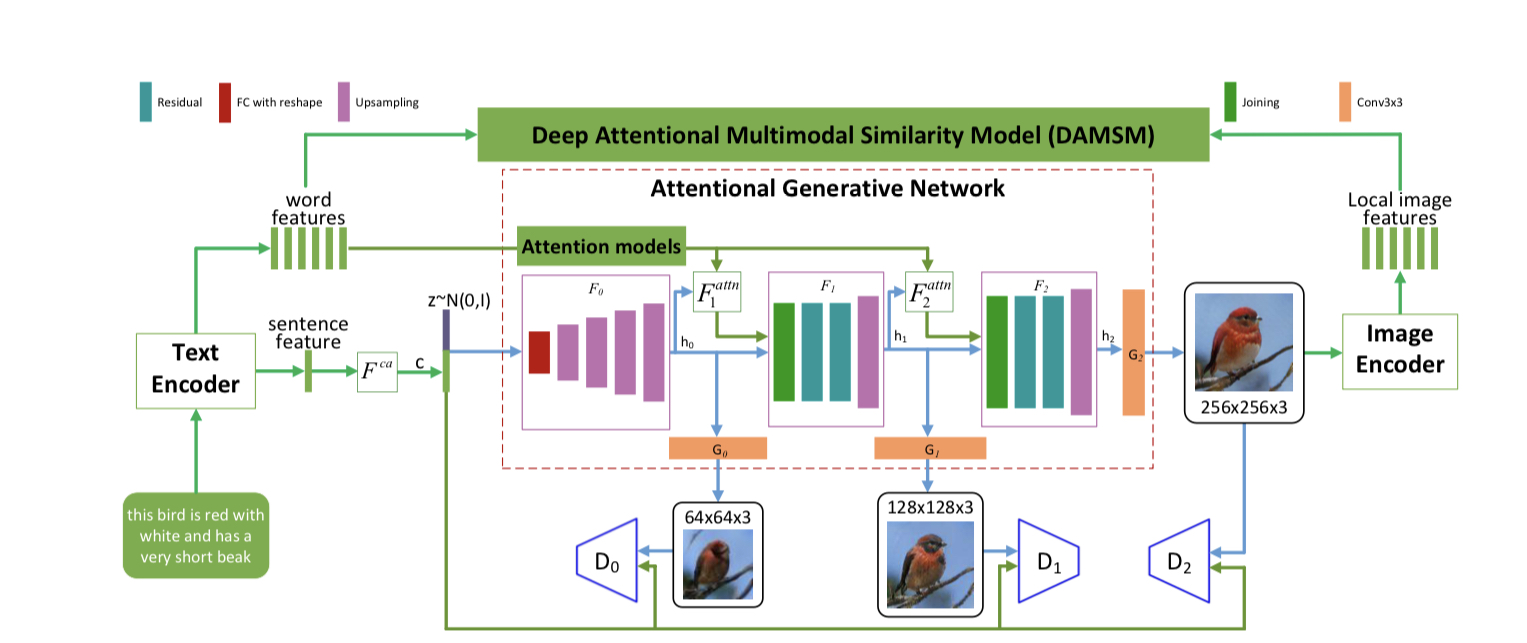
\includegraphics[scale=0.26]{attns} \\
l' AttnGan (Attentional Generative Adversarial Network  ) è un implementazione avanzata delle gan che permette di ottenere un risultato migliore nella generazione di immagini da frasi rispetto a una semplice GAN,in quanto invece che porre tutta la frase descrittiva in un unico vettore  include  tutta una serie di modelli che permettono l'analisi delle singole parole all'interno delle frase presa in cosiderazione;non ostante ottimi risultati siano stati ottenuti anche con il solo vettore descrittivo,questo sistema permette di avere immagini con una grana più fine e con dettagli più versoimili.Una AttnGan presneta due nuovi componenti Una rete generativa attenzionale ( attentional generative network) e il DAMSM (Deep Attentional Multimodal Similarity Model).

\subsubsection{Attentional Generative Network}
gli odierni modelli di GAN per la generazione da testo a immagine  [20, 18, 36, 37] solitamente codificano tutto il testo descrittivo (la frase) in un singolo vettore come condizione per la generazione,un modello del genere pero manca delle informazioni a livello di parola. In questa sezione vediamo un modello che permette di disegnare differenti sottoregioni dell' immagine grazie all' condizionamento sulle parole più rilevanti per quella regione;
avremo quindi n generatori (G0,G1,...Gn-1)
che prendono gli stati (h0,h1,hn-1)come input
e generano immagini di varie dimensioni  (x). 
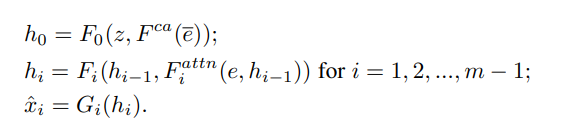
\includegraphics[scale=0.7]{functions}

qui, z è il vettore rumore solitamente campionato da una distribuzione standard
 e(barra) è il vettore che contine tutta la frase,mentre  e è
la matrice dei vettori parola. 
F$^{ca}$ represents the Conditioning
Augmentation [36] that converts the sentence vector e to the
conditioning vector. F$^{attn}$
i
is the proposed attention model
at the i
th stage of the AttnGAN. F
ca
, F
attn
i
, Fi
, and Gi are
modeled as neural networks.
The attention model F
attn(e, h) has two inputs: the
word features e ∈ R
D⇥T
and the image features from the
previous hidden layer h ∈ R
Dˆ⇥N . The word features are
first converted into the common semantic space of the image features by adding a new perceptron layer, i.e., e
0 = Ue,
where U ∈ R
Dˆ⇥D. Then, a word-context vector is computed for each sub-region of the image based on its hidden
features h (query). Each column of h is a feature vector of
a sub-region of the image. For the j
th sub-region, its wordcontext vector is a dynamic representation of word vectors
relevant to hj , which is calculated by
cj =
T
X−1
i=0
βj,ie
0
i
, where βj,i =
exp(s
0
j,i)
PT −1
k=0 exp(s
0
j,k)
, (2)
s
0
j,i = h
T
j
e
0
i
, and βj,i indicates the weight the model attends
to the i
th word when generating the j
th sub-region of the
image. We then donate the word-context matrix for image
feature set h by F
attn(e, h)=(c0, c1, ..., cN−1) ∈ R
Dˆ⇥N .
Finally, image features and the corresponding word-context
features are combined to generate images at the next stage.
To generate realistic images with multiple levels (i.e.,
sentence level and word level) of conditions, the final objective function of the attentional generative network is defined
as
L = LG + λLDAMSM, where LG =
mX−1
i=0
LGi
. (3)
Here, λ is a hyperparameter to balance the two terms of
Eq. (3). The first term is the GAN loss that jointly approximates conditional and unconditional distributions [37]. At
the i
th stage of the AttnGAN, the generator Gi has a corresponding discriminator Di
. The adversarial loss for Gi
is
defined as
LGi = −
1
2
Exˆi∼pGi
[log(Di(ˆxi)]
| {z }
unconditional loss
−
1
2
Exˆi∼pGi
[log(Di(ˆxi, e)]
| {z }
conditional loss
,
(4)
where the unconditional loss determines whether the image
is real or fake while the conditional loss determines whether
the image and the sentence match or not.
Alternately to the training of Gi
, each discriminator Di
is trained to classify the input into the class of real or fake
by minimizing the cross-entropy loss defined by
LDi = −
1
2
Exi∼pdatai
[log Di(xi)] −
1
2
Exˆi∼pGi
[log(1 − Di(ˆxi)]
| {z }
unconditional loss
+
−
1
2
Exi∼pdatai
[log Di(xi, e)] −
1
2
Exˆi∼pGi
[log(1 − Di(ˆxi, e)]
| {z }
conditional loss
,
(5)
where xi
is from the true image distribution pdatai
at the
i
th scale, and xˆi
is from the model distribution pGi
at the
same scale. Discriminators of the AttnGAN are structurally
disjoint, so they can be trained in parallel and each of them
focuses on a single image scale.
The second term of Eq. (3), LDAMSM, is a word level
fine-grained image-text matching loss computed by
